\chapter{Detekcia a rozpoznanie tváre}
\label{kap:detekcia_tvare}
Detekcia a rozpoznanie tváre je aj dnes stále zaujímavá téma v oblasti počítačového videnia. 
Vďaka širokej možnosti využitia v komerčných, bezpečnostných ale aj iných oblastiach 
neustále rastú požiadavky na presnosť, spoľahlivosť a rýchlosť detegovania ľudských tvárí, a to najmä vo videozáznamoch.
Bezpečnostné zložky vedia technológiu využiť na rozpoznanie potenciálne nebezpečnej osoby v dave ľudí alebo zistenie, či sa daná osoba nachádzala na určitom mieste.
V komerčnej oblasti má technológia zasa využitie napríklad na detekciu zákazníkov v podnikoch a podobne. 
Príkladom môže byť systém OptimEyes integrovaný do televízorov vystavených v obchodoch, ktorý deteguje vek, pohlavie a rasu osoby prechádzajúcej popri televízore 
a následne vie podľa získaných informácií prehrať relevantnú reklamu pre tohto zákazníka.\par

Aj keď výskum v tejto oblasti začal už v šesdesiatych rokoch minulého storočia,
stále nebol nájdený dostatočne úspešný prístup k riešeniu problému detekcie a rozpoznávania tváre.
Táto skutočnosť je zjavná, keď porovnáme automatizované systémy na detekciu alebo rozpoznávanie tváre k schopnosti rozpoznávania tvárí u ľudí.
Ľudský mozog dokáže rozpoznať známu tvár v zlomku sekundy. 
Zlé svetelné podmienky, uhol, pod ktorým tvár vidime, zmeny na tvári spôsobené starnutím a podobne našu schopnosť rozpoznať tvár ovplyvňujú len minimálne.
Vieme rozpoznať známu tvár, aj keď je jej časť zakrytá. 
Žiadny existujúci automatizovaný systém nedokáže tváre správne rozpoznať v tomto rozsahu.

\section{Pôvodné spôsoby rozpoznávania tváre}
Pri rozpoznávaní tváre boli spočiatku využívané jej najvýznamnejšie črty. 
Snaha bola vytvoriť systém, ktorý bude rozpoznávať tváre podobným spôsobom, ako človek.
Systém sa snažil určiť dôležitosť niektorých čŕt (oči, ústa, nos) a taktiež vzdialeností medzi nimi.
Tento problém je relevantný aj dnes, pretože ignorovanie niektorých čŕt môže zlepšiť presnosť rozpoznia tváre.
Niektoré nepodstatné časti tváre pôsobia len ako šum.

Avšak abstraktné matematické nástroje ako eigenfaces umožnili pri rozpoznávaní tvári tvári uplatniť aj iné spôsoby.
Vďaka nim je možné porovnať rozdiely medzi dvoma tvárami aj bez sústredenia sa na črty tváre, ktoré pri rozpoznávaní tváre využíva človek.
Niektoré tieto črty sa však aj naďalej využívajú. Príkladom môže byť napríklad farba pleti.

\begin{figure}[H]
\centerline{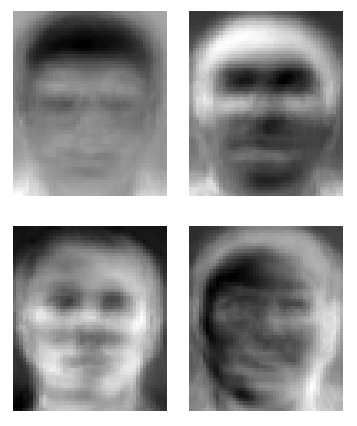
\includegraphics[width=0.6\textwidth]{images/Eigenfaces}}
\caption[Eigenfaces]{Príklad Eigenfaces}
\label{obr:Eigenfaces}
\end{figure}

\section{Systém na rozpoznávanie tváre}
Problém rozpoznania tváre zahŕňa viacero podproblémov. 
Vstupom pre systém na rozpoznanie tváre je buď statický obraz alebo video. 
Výstupom je identifikácia alebo verifikácia osoby alebo osôb nachádzajúcich sa na vstupe.
Proces rozpoznania tváre pozostáva z 3 hlavných krokov. 

\begin{figure}[H]
\centerline{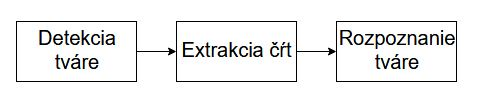
\includegraphics[width=0.8\textwidth]{images/3step}}
\caption[Všeobecný systém na rozpoznávanie tváre]{Všeobecný systém na rozpoznávanie tváre}
\label{obr:3step}
\end{figure}

Detekciu tváre môžme definovať ako proces extrakcie tváre zo scény (vstupu). 
Systém musí správne identifikovať región na vstupe, v ktorom sa nachádza tvár.
V ďalšom kroku, extrakcii čŕt, sa získavajú relevantné črty z dát získaných z predchádzajúceho kroku - detekcie tváre.
Tieto črty môžu byť napríklad isté časti tváre, uhly alebo vzdialenosti medzi nimi.
Nakoniec systém rozpozná tvár. 
Ak je úlohou identifikácia človeka, systém má vrátiť indentitu z nejakej databázy známych ľudí. 
Táto fáza zahŕňa porovnávacie metódy, klasifikačné algoritmy a meranie presnosti detekcie.

\section{Detekcia tváre}
Niektoré aplikácie tento krok nevyžadujú. 
Dôvodom je, že v databáze zväčša už máme uložené podobizne tvári známych ľudí v normalizovanej forme.
Vstupné dáta do systému majú v týchto aplikáciach tiež nejaký štandardný formát. 
Príkladom môže byť napríklad databáza hľadaných zločincov. 
Pri zisťovaní, či sa osoba v danej databáze už nachádza, použijeme štandardnú fotku tváre spredu a tým pádom detekcia tváre nie je potrebná.
Pre všeobecný systém na respoznávanie tváre však nemôžeme klásť požiadavku na štandardný vstup.
Na vstupe sa môže nachádzať viacero tvárí alebo iných objektov a to na rôznych miestach, pod rôznymi uhlami a podobne.
Príkladom nakéhoto systému by mohli byť napríklad bezpečnostné kamery na verejnom mieste, ktoré by mali zaistiť, že sa na danom mieste nenachádza žiadna osoba nachádzajúca sa v databáze hľadaných zločincov.
Preto je rozumné zahrnúť detekciu tváre medzi kroky rozpoznania tváre.

\subsection{Problémy a výzvy pri detekcii tvárí}
Ako už bolo spomenuté, na systém nechceme klásť žiadne podmienky na štandardný vstup.
Preto sa musíme vedieť vysporiadať s niekoľkými výzvami, ktoré zväčša vznikajú v nekontrolovanom prostredí, ako je napríklad verejný priestor sledovaný bezpečnostnými kamerami.
Problémy vznikajú pri nasledujúcich situáciach.

\begin{description}
  \item[Uhol tváre] 
  Ideálna situácia by bola, keby každú tvár vidíme vždy spredu, alebo aspoň vždy pod rovnakým uhľom. 
  V reálnom nekontrolovanom prostedí je však táto požiadavka nereálna, tvár vidíme pod rôznymi uhlami kvôli umiestneniu kamier alebo kvôli samotnému pohybu sledovanej osoby.
  Navyše rastie aj výpočtová sila potrebná pre detekciu tváre v závislosti od uhlu, pod ktorým tvár vidíme.
  \item[Zakrytie tváre] Tvár nemusí byť vždy viditeľná celá, jej časť môže byť napríklad prekrytá okuliarmi, šálom, fúzami, prípadne aj inými objektami nachádzajúcime sa v scené vrátene ďalších tvárí.
  \item[Výraz tváre] Výraz tváre taktiež môže zťažiť detekciu tváre. Pri rôznych výrazoch tváre sa výrazne menia viaceré črty tváre, ich pozícia na tvári, uhol a podobne.
  \item[Problémy súvísiace so zachytením obrazu] Obraz zachytení kamerami sa môže líšiť v závislosti od typu kameri, jej nastavení, osvetlení prostredia, hmle a podobne.
\end{description}

\subsection{Lokalizácia tváre}
Pri lokalizácii tváre je cielom zistiť pozíciu tváre, keď na vstupe je práve jedna tvár. 
Ide v podstate o zjednodušenú formu detekcie tváre.
Metódy ako hľadanie hranice tváre boli pôvodne používané na riešenie tohto problému.
Detekcia čŕt tváre je používaná na hľadanie a lokalizovanie niektorých relevantných čŕt tváre, ako sú oči, nos, ísta, pery, uši a tak ďalej.
Niektoré algoritmy na extrakciu čŕt tváre sú založené práve na detekcii čŕt tváre.
Sledovanie tváre je ďalším problémom odvodeným z detekcie tváre. 
Cieľom viacerých systémov je nie je len detegovať tvár, ale zároveň je vedieť aj lokalizovať v reálnom čase. 
Bezpečnostné kamery sú opäť dobrým príkladom.

\begin{figure}[H]
\centerline{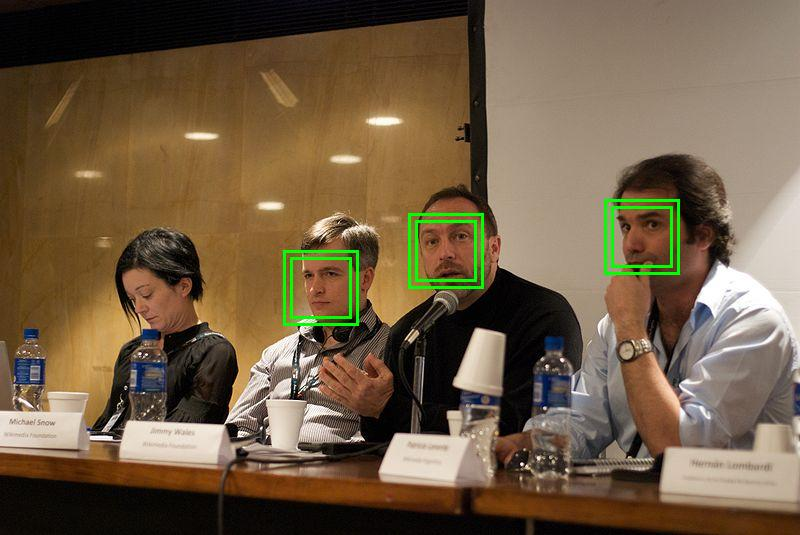
\includegraphics[width=0.8\textwidth]{images/detection_v}}
\caption[Detekcia tvára]{Vizualizácia detekcie a lokalizácie tváre. Systému sa správne podarilo detegovať a lokazolizovať
tri zo štryroch tvárí na obrázku. Môžme si všimnúť, že systém tváre dokázal detegovať pod rôznymi uhlami aj keď je malá časť tváre zakrytá.}
\label{obr:3step}
\end{figure}

\subsection{Štruktúra problému detekcie tváre}
Detekcia tváre je problém, ktorý je taktiež zložený z viacerých podproblémov.
Niektoré systémy na detekciu tváre  detegujú a lokalizujú tvár naraz, 
iné najskôr vykonajú detekciu tváre a ak sa zistí, že na vstupe sa nachádza tvár, tak potom sa snažia túto tvár lokalizovať.
Potom sa môžu využiť aj iné algoritmy na sledovanie tváre. 
Rôzne algoritmy na detekciu tváre často zdieľajú rovnaké alebo veľmi podobné kroky.
Najskôr sú dáta na vstupe zmenšené. Zmenšenie dát spôsobí rýchlejší beh algoritmu.
Potom môžu byť vstupné dáta nejakým spôsobom predspracované, aby napríklad spĺňali podmienky pre vstup algoritmu.
Po tomto kroku niektoré algoritmy analyzujú vstup tak, ako sme ho po predchádzajúcich dvoch krokoch dostali.
Iné algoritmy sa môžu pokúšať extrahovať z dát nejaké relevantné regióny tváre. 
Tie potom budú vyhodnotené a porovnané aby sa určilo, či sa na vstupe nachádzala tvár ak ak áno, tak kde.
Nakoniec niektoré algoritmy využívajúce strojové učenie pridajú nové dáta do svojho modelu.

Detekcia tváre je problém druhu binárnej klasifikácie (dve triedy - ??? preklad) (musíme rozhodnúť, či sa na vstupe nachádza alebo nenachádza tvár.)
Tento postup môžme označiť aj ako zjednodušenú verziu problému rozpoznávania tváre. 
Systém na rozpoznávanie tváre musí klasifikovať danú tvár na vstupe, pričom toľko tried klasifikácie (??? - opäť preklad), koľko je kandidátov, teda známych tvári v databáze.
Preto sú mnohé metódy na detekciu tváre podobné algoritmon na rozpoznávanie tváre. 
Techniky používané na detekciu tváre sú často použivané pri rozpoznávaní tváre.

\section{Postupy využívané na detekciu tváre}
Nie je jednoduché rozdeliť postupy na detekciu tváre do samostnatných nezávislých kategórií.
Častu sú v jednom algoritme využívané viaceré, prote sa kategórie môžu prekrývať.
Popíšeme dve klasifikačné kritéria. V prvom z nich rozlišujeme medzi rôznymi scenármi.
V druhom je problém detekcie dváre rozdelený do štyroch kategórií.
 

\subsection{Detekcia tváre závislá na scenári}
\begin{description}
  \item[Kontrolované prostredie] 
  Jedná sa o najjednoduchší prípad. Fotografie alebo videá sú zachytené v kontrolovanm prostredí.
  To znamená, že vždy bude osvletlenie scény rovnaké, pozadie bude vždy to isté a podobne.
  Na detekciu tváre v tomto prípade môžme použiť jednoduchú detekciu hrán.
  \item[Farebné obrázky/videá]
  Typická farba pokožky môže byť použitá na nájdenie tváre. 
  Problém môže nastať, pokiaľ sa menia svetelné podmienky. 
  Navyše farba ľudskej pokožky sa môže výrazne líšiť, od takmer bielej až po takmer čiernu.
  Ako sa však ukazuje, toto pri detekcií nie je až taký veľký problém.
  Napriek tomu je ťažké ustanoviť nejakú silnú reprezentáciu ľudskej kože.
  Existujú však pokusy o vytvorenie robustného systému na detekciu tváre, ktorý by práve využíval farbu pokožky.
  \item[Videá]
  Videá nám dávajú viacej informácií, ako len obrázky. 
  Preto je pri detekcii tváre vo videu využiť techniky detegujúce pohyb na lokalizáciu tváre.
  Existujú systémy, ktoré využívajú pohyb viečok pri žmurkaní na detekciu tváre.
  Takéto systémy však vyžadujú vysokú kvalitu vstupných dát.
\end{description}

\begin{figure}[H]
\centerline{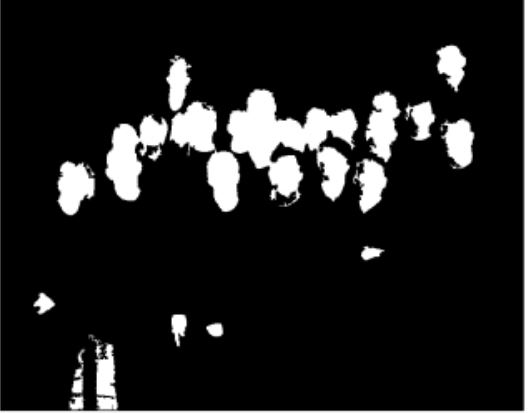
\includegraphics[width=0.8\textwidth]{images/skin}}
\caption[Detekcia tvára]{Výsledok farebnej segmentácie}
\label{obr:skin}
\end{figure}

\begin{figure}[H]
\centerline{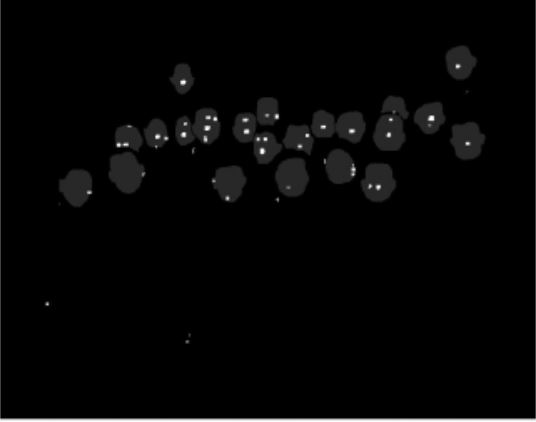
\includegraphics[width=0.8\textwidth]{images/template}}
\caption[Detekcia tvára]{Výsledok template matchingu použítím templatu pre oči a tváre}
\label{obr:template}
\end{figure}

\subsection{Detekcia tváre rozdelená do štyroch kategórií}
Yan, Kriegman a Ahuja predstavili klasifikáciu, ktorá je celkom dobre akceptovaná odborníkmi z oblasti.
Metódy na detekciu tváre rozdelili do štyroch kategórií, pričom sa však tieto kategórie môžu prekrývať, takže algoritmy môžu patriť aj do viacerých kategórií naraz.
Klasifikácia vyzerá nasledovne.
\begin{description}
  \item[Metódy založené na vedomostiach] 
  Patria sem metódy založené na pravidlách, ktoré využívajú naše znalosti o ľudských tvárach.
  \item[Metódy využívajúce nemenné črty]
  Metódy sa snažia nájsť nemenné znaky/črty tváre a to bez ohľadu na ich pozíciu alebo uhol.
  \item[Metódy využívajúce template matching]
  Tieto algoritmy porovnajú vstupný obraz s vopred uloženými vzorkami alebo črtami tváre.
  \item[Metódy založené na výskyte]
  Sú to metódy využívajúce template matching, ale databáza vzoriek vznikne učením sa na sade trénovacích obrázkov.
\end{description}

\subsection{Metódy založené na výskyte (Appearance-based methods)}
Vzorky su v metódach založených na výskyte naučené z príkladov v trénovacích obrázkoch.
Vo všeobecnosti metódy založené na výskyte sa zakladajú na technikách zo štatistickej analýzy a strojového učenia
na nájdenie relevantných charakteristík na obrázku tváre.
Niektoré metódy založené na výskyte pracujú v pravdepodobnostných sieťach.
Funkčný vektor je náhodná premenná určujúca pravdepodobnosť, že daný vektor patrí nejakej tvári alebo nie.
Ďalší existujúci spôsob je definovať diskriminačnú funkciu medzi triedami tvár a nie-tvár.
Takéto metódy sú využívané pri extrakcii čŕt pri rozpoznávaní tváre.
Existujú viaceré relevantné nástroje a metódy.
\begin{description}
  \item[Založené na eigenface] 
  Sirovich and Kirby vyvinuli metódu na efektívnu reprezentáciu tvárí s využitím PCA (Principal Component Analysis).
  Ich cieľom bolo reprezentovať tvár ako súradnicový systém.
  Vektory, ktoré tvoria tento súradnicový systém sa nazývajú eigenpictures. 
  Turk and Pentland neskôr využili tento postup a vyvinuli algoritmus založený na eigenface na rozpoznávanie tváre.
  \item[Založené na distribúcii]
  Tieto systémy boli najskôr používane na detekciu objektov a patternov.
  Princípom je zozbierať dostatočne veľký počet vzoriek pre triedu patternu, ktorý chceme detegovať.
  ...
  \item[Neurónové siete]
  Veľa problémov rozpoznávania patternov sa dá úspešne riešiť neurónovými sieťami.
  Neurónová sieť sa dá použiť na naučenie patternov pre tvár a ne-tvár.
  Problémom je reprezentácia triedy, ktorá reprezentuje patterny bez tváre.

\end{description}

\section{Sledovanie tváre}
Množstvo systémov na rozpoznávanie tváre má ako vstup video. Pre tieto systémy môže byť užitočné okrem detekcie tváre túto tvár aj sledovať.
Na sledovanie tváre môže byť použité množstvo rôznych metód, napríklad sledovanie hlavy, sledovanie jednotlivých čŕt tváre a iné.
Základný princíp je na začiatku detegovať tvár a následne zistiť rozdiely medzi jednotlivými snímkami a aktualizovať pozíciu tváre.
Podobne ako pri detekcii treba riešiť rôzne problémy. Napríklad čiastočné zakrytie tváre, zmena osvetlenia, rýchlosť výpočtu, deformácia tváre.
Príkladom algoritmu na sledovanie tváre je algoritmus, kde stavový vektor tváre obsahuje pozíciu stredu obrázku, veľkosť oblžníku obsahujúceho tvár, priemernú farbu oblasti tváre.
Noví kandidáti na tvár sú vypočítaní pomocou Kalmanovho filtra. Pri sledovaní, ak tvár nie je nová, tak tvár z predchádzajúcej snímky sa použije ako template.
Pozícia tváre je vypočítaná pomocou Kalmanovho filtra and región tváre je prehľadaná SSD algoritmom použitím tohto templatu.
Keď SSD nájde región, informácia o farbe je vložnená do Kalmanovho filtra pre presné nájdenie hranice regiónu tváre.
Potom je aktualizovaný stavový vektor.
Uvedený algoritmus ukazuje dobré výsledky aj keď sa niektoré tváre prekrývajú alebo keď sa mení osvetlenie.